    % \documentclass[handout,xcolor=pdftex,dvipsnames,table]{beamer}
    \documentclass{beamer}

    \usepackage{amsmath}
    \usepackage[english,brazil]{babel}
    \usepackage[utf8x]{inputenc}
    \usepackage{graphicx}
    \usepackage{url,color,ae}
    \usepackage{listings,color,upquote}
    \usepackage[T1]{fontenc}
    \usepackage[small]{caption}

    \hypersetup{pdftitle={IFSC - Campus Sao Jose},
	    pdfsubject={Telecomunicacoes}
    }



    %--------- Insercao de codigo fonte nos slides --------------------%
    \definecolor{hellgelb}{rgb}{1,1,0.9}
    \definecolor{colKeys}{rgb}{0,0,0}
    \definecolor{colIdentifier}{rgb}{0,0,0.9}
    \definecolor{colComments}{rgb}{.4,.4,.4}
    \definecolor{colString}{rgb}{0,0,0.6}

    % Comando: \java
    \newcommand{\java}
    {\lstset{language=java,basicstyle=\ttfamily\footnotesize,tabsize=3,frame=single,
    showtabs=false,showspaces=false,firstnumber=last,numbers=left,numberstyle=\tiny,
    linewidth=0.98\linewidth,xleftmargin=21pt,tab=$\to$,float=tbph,extendedchars,
    breaklines,showstringspaces=false,identifierstyle=\color{colIdentifier},
    keywordstyle=\color{colKeys},stringstyle=\color{colString},commentstyle=\color{
    colComments},backgroundcolor=\color{hellgelb},columns=flexible,captionpos=b,
    aboveskip=\bigskipamount}}

    % Comando: \shell
    \newcommand{\shell}
    {\lstset{language=csh,basicstyle=\ttfamily\footnotesize,tabsize=3,frame=single,
    showtabs=false,showspaces=false,firstnumber=last,numbers=left,numberstyle=\tiny,
    linewidth=0.98\linewidth,xleftmargin=21pt,tab=$\to$,float=tbph,extendedchars,
    breaklines,showstringspaces=false,identifierstyle=\color{colIdentifier},
    keywordstyle=\color{colKeys},stringstyle=\color{colString},commentstyle=\color{
    colComments},backgroundcolor=\color{hellgelb},columns=flexible,captionpos=b,
    aboveskip=\bigskipamount}}

    % ------------------ TEMA ---------------------------------------------%

    \usetheme[numbers,totalnumber,compress]{Madrid}
    % \usetheme{Warsaw}
    % \usetheme{Boadilla}
    % \usetheme{CambridgeUS}
    % \usetheme{Montpellier}
    % \usetheme{Hannover}
    % \usetheme{Dresden}


    \definecolor{azulescuro}{rgb}{0.3,0.42,0.601}  
    \definecolor{verde}{rgb}{0.55,0.78,0.25} 
    \definecolor{kugreen}{RGB}{50,93,61}
    \definecolor{kugreenlys}{RGB}{132,158,139}
    \definecolor{kugreenlyslys}{RGB}{173,190,177}
    \definecolor{kugreenlyslyslys}{RGB}{214,223,216}
    
    \usecolortheme[named=kugreen]{structure}
    \useinnertheme{circles}

    \setbeamertemplate{footline}[frame number]
    \beamertemplatenavigationsymbolsempty
    % ------------------------------------------------------------------ %

    \logo{
\includegraphics[width=.5cm]{figs/logo-ifsc.pdf}}






    % -------------------- Titulo -----------------------------------%

    \title{Projeto de instalação de uma emissora de radiodifusão sonora em frequência modulada, no município de São Pedro de Alcântara}
    \subtitle{}
    \author[Guilherme Bilbao Soares da Silva]{Guilherme Bilbao Soares da Silva\\Jaci Destri}
    \institute[IFSC]{
    Instituto Federal de Santa Catarina -- IFSC\\
    Campus São José \\
    \url{}
    }

    \date{Julho de 2013}


    % -------------- Início do documento ------------------ %
    \begin{document}

    \begin{frame}
	    \maketitle
    \end{frame}

    \frame{\frametitle{Conteúdo Programático}
    \tableofcontents}

    %\AtBeginSection[]{
    % \frame{
      %  \frametitle{Índice}
      % \tableofcontents[current,currentsection]
      %}
    %}

    \section{Motivação}
    \begin{frame}
    \frametitle{Motivação}
      \begin{itemize}
      \item Adquirir maiores conhecimentos em radiotransmissão;
      \item Estudo e compreensão das normas técnicas;
	\item A norma técnica sofre adaptações;
	\item Servir como referência para outros projetos/estudos.
	\end{itemize}

    \end{frame}


    \section{Proposta}

    \begin{frame}
	    \frametitle{Proposta}
      \begin{itemize}

	    \item Projeto de uma emissora FM num cenário real,
	    seguindo os procedimentos solicitados pela resolução
	    e normas vigentes para esta finalidade.   
	    Para isto, é utilizado o canal 218 (91,5 Mhz),disponível no plano básico,
	    no município de São Pedro de Alcântara.
	\end{itemize}    
	  
    \end{frame}
    
    \begin{frame}
    
      \frametitle{Proposta}
      \begin{itemize}
      
      \item Objetivos Principais:
      
      
      
      \begin{itemize}
	  
	  \item Elaborar um documento que reúna todas a informações necessárias
	  para encontrar os resultados desejados neste estudo, e que também 
	  auxilie outros projetos similares futuramente.
	    
	  \item Apresentar os dados técnicos solicitados pela 
	    ANATEL, definidos através da Resolução n°67 e suas atualizações;
	    
	    
      \end{itemize}
    \end{itemize} 
    
    \end{frame}

    \section{Desenvolvimento}
      
    \begin{frame}
    
      \frametitle{Desenvolvimento}
      \begin{itemize}
          \item Informações e ferramentas necessárias para o desenvolvimento:
	\begin{itemize}
 
	  \item PBFM;
	  \item Resolução nº 67;
	  \item Recomendação UIT-R P.1546;
	  \item Ferramenta SIGAnatel.
      
      \end{itemize}
  \end{itemize} 
    \end{frame}
    
    \begin{frame}
    
      \frametitle{Desenvolvimento}
      
      \begin{itemize}
      
         \item  Canal proposto:
          
       
          
	\begin{itemize}
	
	  \item Município de São Pedro de Alcântara;
	  \item Canal 218 (91,5 MHz) no PBFM;
	  \item Classe C;
	  \item Contorno protegido de 7,5 Km.
      
      \end{itemize}
   \end{itemize}
    \end{frame}
    
        \begin{frame}
    
      \frametitle{Desenvolvimento}
      
      \begin{itemize}
	 \item Classificação da emissora:
	 
	 \end{itemize}
	 
      \begin{center}
      
           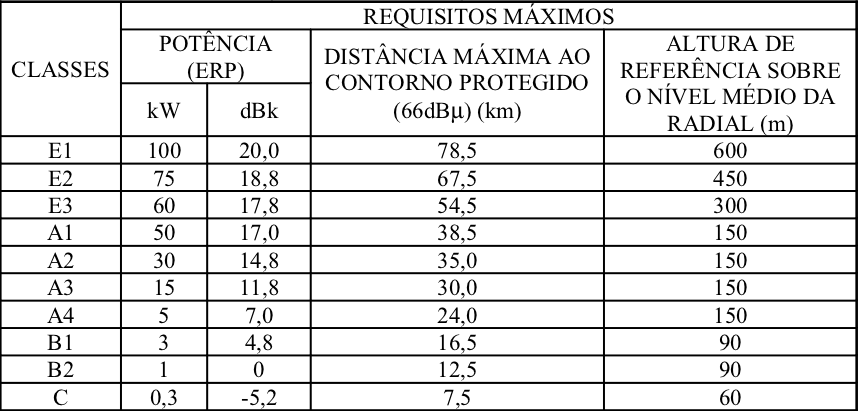
\includegraphics[width=.8\linewidth]{figs/tabelaClassificacaoEmissoras.png}		  		
        \end{center}
      
        
  
	\end{frame}
    
    \begin{frame}
    
      \frametitle{Desenvolvimento}
      
      \begin{itemize}
      
          \item Localização da base emissora:
          
	\begin{itemize}
	

	  \item 27º34'02.72''S, 48º48'33.71''O;
	  \item Área central do município;
	  \item 285 metros de altitude;
	  \item Ponto mais próximo ao local informado no PBFM.
      
      \end{itemize}
   \end{itemize}
    \end{frame}
    
        \begin{frame}
    
      \frametitle{Desenvolvimento}
      
      
      \begin{itemize}

         \item  Sistema irradiante:
          
          
	\begin{itemize}
	

	  \item Antena Dipolo 1/2 onda;
	  \item Trasmissor de 150 Wrms;
	  \item Cabo coaxial, atenuação = 0,680dB/100m;
	  \item Altura da Torre = 55 m.
      
      \end{itemize}
   \end{itemize}
    \end{frame}
    
    \begin{frame}
    
      \frametitle{Desenvolvimento}
      \begin{itemize}
	\item  Obtendo o NMR e o NMT:
      \end{itemize}
     
      \begin{center}
      
           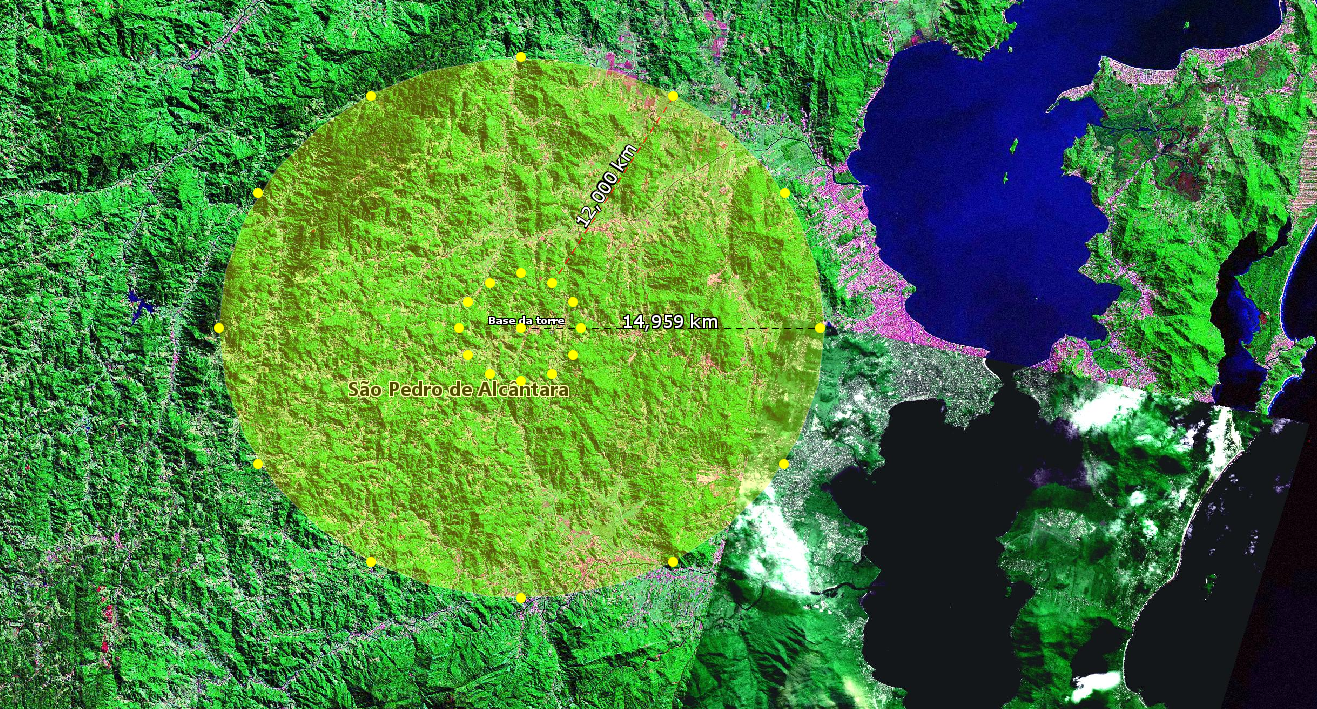
\includegraphics[width=.8\linewidth]{figs/radiais_detalhado.png}		  		
        \end{center}
  
      \end{frame}
    
     \begin{frame}
    
      \frametitle{Desenvolvimento}
      
      \begin{itemize}
	\item Obtendo o NMR e o NMT:
      \end{itemize}
      \begin{center}
      
           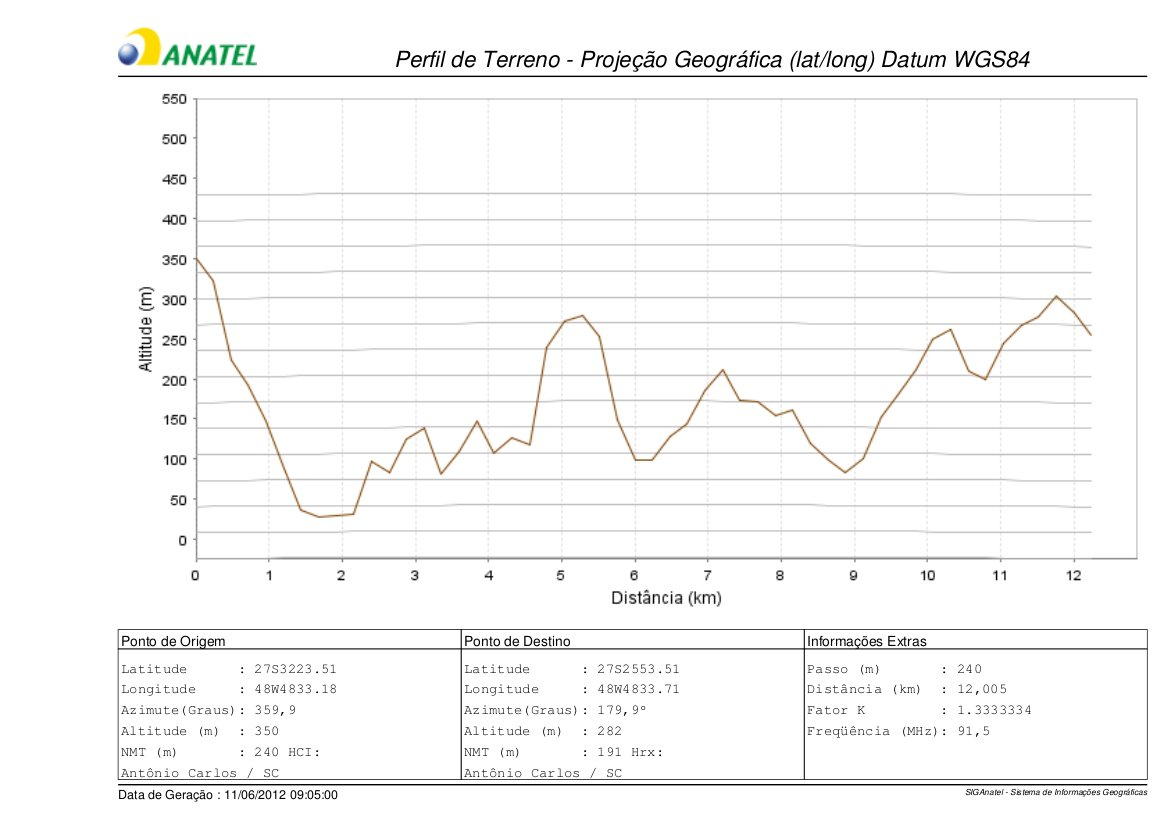
\includegraphics[width=.9\linewidth]{figs/nmt1_v2.jpg}		  		
        \end{center}
  
      \end{frame}
    
    \begin{frame}
    
    
      \frametitle{Desenvolvimento}
      
      \begin{itemize}
     \item Potência Efetiva Irradiada Máxima:

      \begin{itemize}
       \item É composta de variáveis que correspondem aos equipamentos e suas características no sistema;
       
       \item $ERPmax = Pt \times Gtmax \times Ef$.
      \end{itemize}
    \end{itemize}
    \end{frame}
    
       \begin{frame}
    
      \frametitle{Desenvolvimento}
      
      \begin{itemize}
      
      \item Potência Efetiva Irradiada Máxima:
      
       \end{itemize}
       
       $$ERPmax = 0,15 kW \times 3 \times 0,569$$
       $$ERPmax = 0,256 kW$$
        $$ERPmax = -5,91 dBk$$
   
 
    \end{frame}
    
    \begin{frame}
    
      \frametitle{Desenvolvimento}
      
      \begin{itemize}
      
         \item HNMT:
         
         
	\begin{itemize}
	
	  %\item NMT=288,33 metros;
	  %\item Referência para definir altura da antena;
	  \item HCGSI = 55m + 4,244m
	  \item HNMT = CBT + HCGSI - NMT
	  \item 55,914 = 285m + 59,244 - 288,33m
      
      \end{itemize}
   \end{itemize}
    \end{frame}
    
        \begin{frame}
    
      \frametitle{Desenvolvimento}
      
      \begin{itemize}
      
      \item Valores de HNMT para cada radial:
      
      
       \end{itemize}
      \begin{center}
      
          \def\tablename{Tabela}
      \begin{table}
	\vspace*{0.05cm}
	\centering

	\begin{tabular}{|c|c|c|} \hline

	  Radial (graus) & NMR (m) & HNMT (m)\\ \hline
	  0° & 158,38&185,86\\
	  30° & 73,46 & 270,78\\
	  60° & 169,14 & 175,10\\
	  90° & 166,20 & 178,04\\
	  120° & 250,46 & 93,78\\
	  150° & 196,86 & 147,38\\
	  180° & 151,58 & 192,66\\
	  210° & 394,80 & -50,55\\
	  240° & 502,10 & -157,85\\
	  270° & 579,60 & -235,35\\
	  300° & 412,10 & -67,85\\
	  330°& 405,32 & -61,07\\ \hline

	\end{tabular}
      \end{table}		  		
      \end{center}
  
  
    \end{frame}
    
    
    
    
    \begin{frame}
    
      \frametitle{Desenvolvimento}
      
      \begin{itemize}
            
      \item Diagrama de irradiação de Antena:
      
      \end{itemize}
	 
      \begin{center}
      
           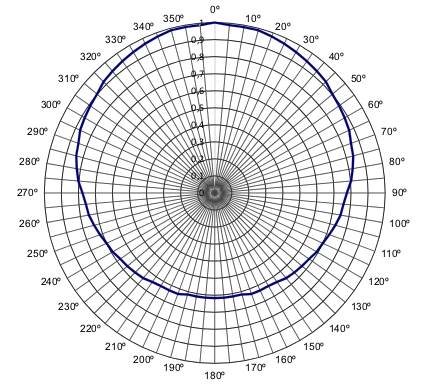
\includegraphics[width=.6\linewidth]{figs/diagrama_de_irradiacao.jpg}	
           
        \end{center}
      
      
  
  \end{frame}
  
      \begin{frame}
    
      \frametitle{Desenvolvimento}
      
      \begin{itemize}
      
      \item Valores de ERPaz para cada radial:
      
       \end{itemize}
	 
      \begin{center}
      
     \def\tablename{Tabela}
	  \begin{table}
	  \vspace*{0.05cm}
	  \centering

	      \begin{tabular}{|c|c|c|c|} \hline

	      Radial & E/Emax & ERPaz(kW) & ERPaz(dBk)\\\hline\hline
	      $0°$  & 0,78 & 0,1560 & -8,07 \\\hline
	      $30°$ & 0,69 & 0,1220 & -9,13 \\\hline
	      $60°$ & 0,63 & 0,1017 & -9,92 \\\hline
	      $90°$ & 0,62 & 0,0985 & -10,06 \\\hline
	      $120°$& 0,63 & 0,1017 & -9,92 \\\hline
	      $150°$& 0,69 & 0,1220 & -9,13 \\\hline
	      $180°$& 0,78 & 0,1560 & -8,07 \\\hline
	      $210°$& 0,88 & 0,1985 & -7,02 \\\hline
	      $240°$& 0,95 & 0,2314 & -6,35 \\\hline
	      $270°$& 1,00 & 0,2564 & -5,91 \\\hline
	      $300°$& 0,95 & 0,2314 & -6,35 \\\hline
	      $330°$& 0,88 & 0,1985 & -7,02 \\\hline

	      \end{tabular}
	
	  \label{tabelaERPaz}
	  \end{table}	
           
        \end{center}
      
      
  
  \end{frame}
  
      \begin{frame}
    
      \frametitle{Desenvolvimento}
      
       \begin{itemize}
      
      \item Definindo os contornos: 
      
       \end{itemize}
      \begin{center}
      
           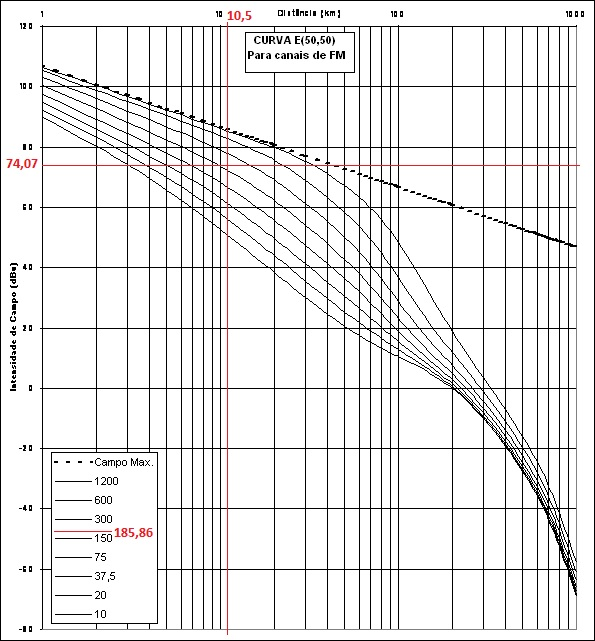
\includegraphics[width=.6\linewidth]{figs/e5050_calc.jpg}	
           
        \end{center}
      
  \end{frame}
  
  
      \begin{frame}
    
      \frametitle{Desenvolvimento}
      
      \begin{itemize}
      
      \item Distâncias do contorno protegido (66 dBm):
      
      \end{itemize}
      
      \begin{center}
  
	  \def\tablename{Tabela}
	  \begin{table}
	  \vspace*{0.05cm}
	  \centering

	  \begin{tabular}{|c|c|c|c|c|} \hline

	  Radial& ERPaz(dBk) & HMNT (m) & 66 dBm & Contorno 2 (km)\\\hline\hline
	  $0°$  & -8,07 &185,86 &74,07 &10,5\\\hline
	  $30°$ & -9,13 &270,78 &75,13 &11  \\\hline
	  $60°$ & -9,92 &175,10 &75,92 &9   \\\hline
	  $90°$ & -10,06&178,04 &76,06 &9   \\\hline
	  $120°$& -9,92 &96,78  &75,92 &7   \\\hline
	  $150°$& -9,13 &147,38 &75,13 &9   \\\hline
	  $180°$& -8,07 &192,66 &74,07 &11  \\\hline
	  $210°$& -7,02 &-50,55 &73,02 &3,2 \\\hline
	  $240°$& -6,35 &-157,85&72,35 &3,4 \\\hline
	  $270°$& -5,91 &-235,35&71,91 &3,6 \\\hline
	  $300°$& -6,35 &-67,85 &72,35 &3,4 \\\hline
	  $330°$& -7,02 &-61,07 &73,02 &3,2 \\\hline

	  \end{tabular}
	  \label{tabelaContorno2}
	  \end{table}
	      
    
            \end{center}
      
  \end{frame}
  
          \begin{frame}
    
      \frametitle{Desenvolvimento}
      
      \begin{itemize}

      \item Áreas de cobertura:

      \end{itemize}
      
      \begin{center}
      
           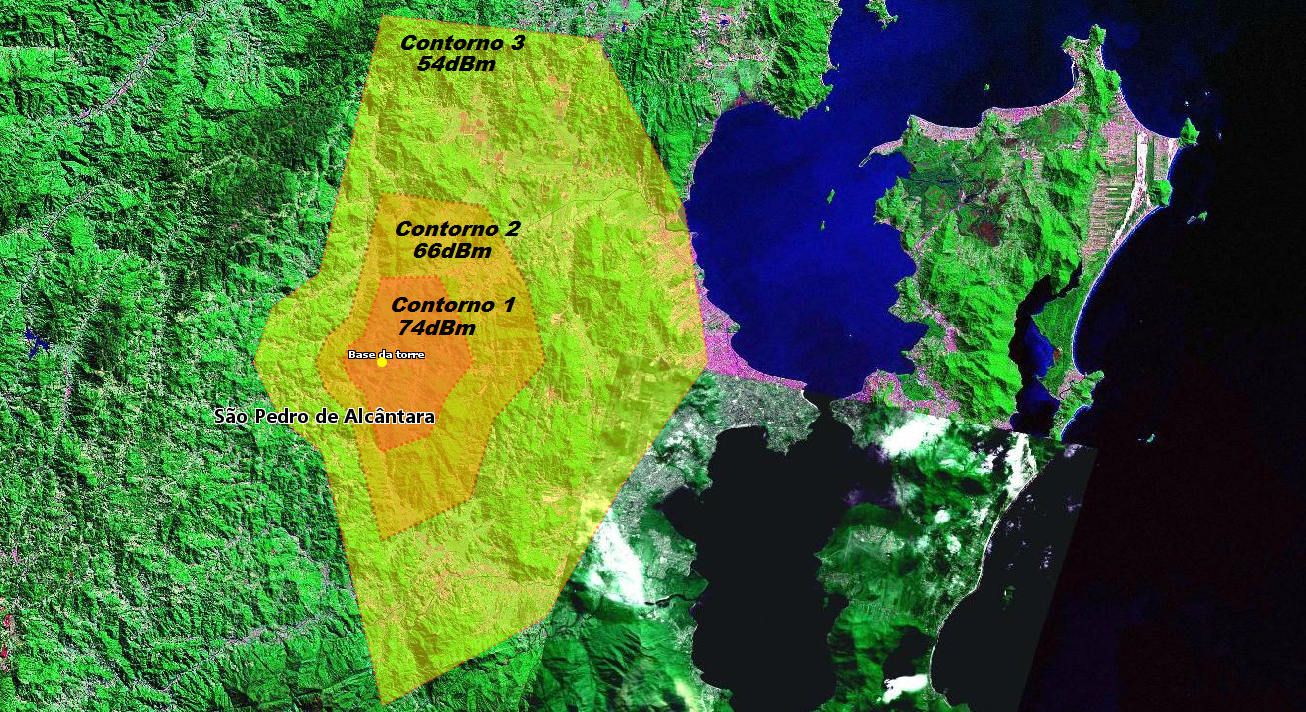
\includegraphics[width=.8\linewidth]{figs/todososcontornos.png}	
           
        \end{center}
      
  \end{frame}
 
   % \begin{center}
    %\begin{array}{ll}
    %\includegraphics[width=.5\linewidth]{figuras/fou.png}		  		
    %\caption{}  & \includegraphics[width=.5\linewidth]{figuras/wa.png}		
    %  \caption{} 
    %\end{array}
    %\end{center}

    
    
    \section{Resultados}
    
     \begin{frame}
    
      \frametitle{Resultados}
      
      \begin{itemize}
      
      \item Obediência aos requisitos máximos (classe C):
     
      
	\begin{itemize}

	  \item ERPmax = 0,256kW < 0,3kW;
	  \item Altura de referência sobre o nível médio do terreno = 55,914m < 60m;
	  \item Contorno protegido (66dBm) = 6,942km < 7,5km.
      
      \end{itemize}
   \end{itemize}
    \end{frame}
    
    
        \begin{frame}
    
	\frametitle{Resultados}
      \begin{itemize}
      
         \item Cobertura da área central e urbana do município:
      \end{itemize}
	  \begin{center}
      
           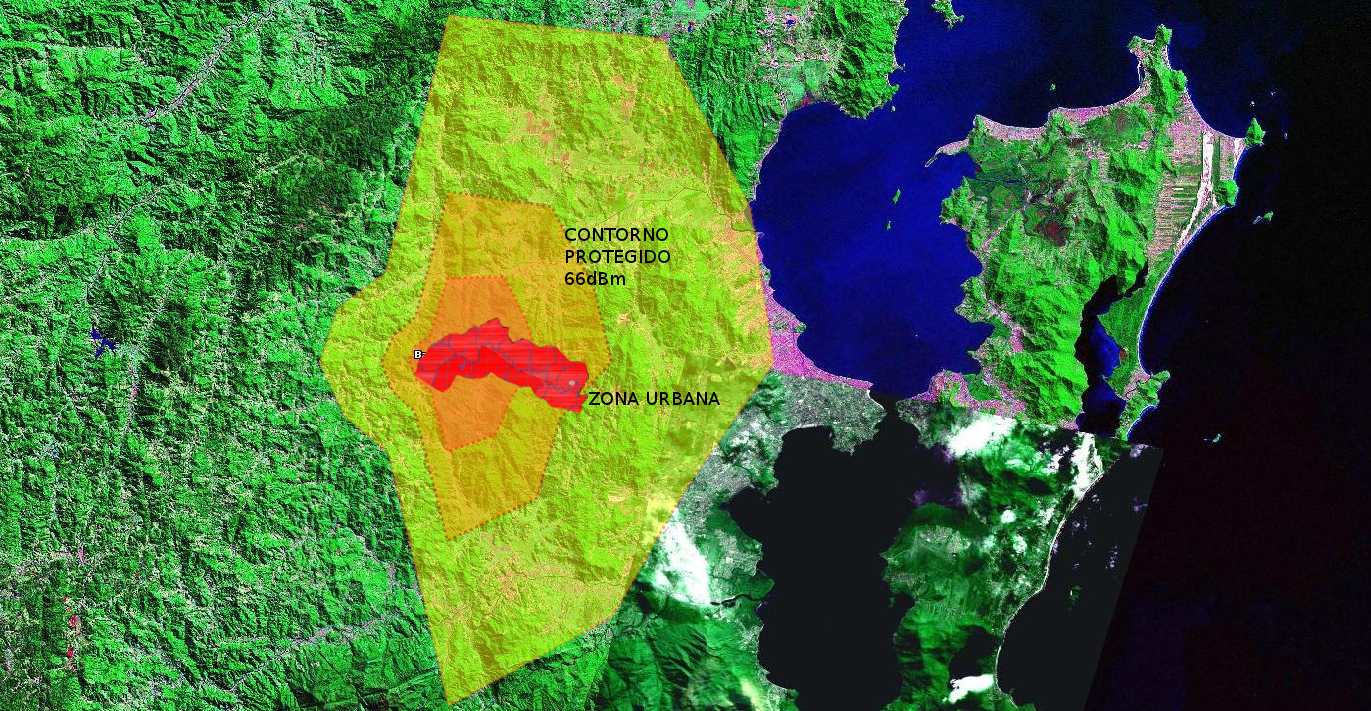
\includegraphics[width=.8\linewidth]{figs/contornoAreaUrbana.png}	
           
	  \end{center}
      
	\end{frame}

    \section{Conclusões}
    \begin{frame}
    \frametitle{Conclusões}
    
    \begin{itemize}
    
    \item Conclusões específicas do projeto:
   
    \begin{itemize}
    \item Todos os requisitos técnicos relacionados à classe da emissora foram atendidos;
    \item Comprovada a viabilidade técnica do canal para o município (relação área urbana/classe da emissora);
    \item Similaridade com os resultados apresentados pela ferramenta SIGAnatel.
    \end{itemize}
    \end{itemize}
    \end{frame}
    
    \begin{frame}
    \frametitle{Conclusões}
    
    \begin{itemize}
    
    \item Conclusões gerais:
    
      \begin{itemize}
    \item A combinação de diversas configurações diferentes (elementos) pode apresentar os mesmos resultados (cobertura);
    \item O relevo da região é o fator que mais gera influência na escolha dos elementos usados na configuração da emissora.
      \end{itemize}
    \end{itemize}
    \end{frame}

    \section{Trabalhos Futuros}
    \begin{frame}
    \frametitle{Trabalhos Futuros}
    
	    \begin{itemize}
     
	    \item Sugestões:

	    
	    \begin{itemize}
		  \item Simulação computacional de estudo de viabilidade técnica implementado no Matlab, baseado nos métodos apresentados na Recomendação UIT-R P.1546;

		  \item Projeto de viabilidade técnica para alteração da classe da emissora, com a finalidade de aumento da àrea de cobertura;

   
    \end{itemize}
    \end{itemize}
    \end{frame}

    \begin{frame}

      \frametitle{Obrigado pela atenção!}
      
      \begin{center}
      
    {\huge Dúvidas? } 

      \end{center} 
    
    \end{frame}

    \end{document}
